% !TeX root=../main.tex

\chapter{مقدمه}
% دستور زیر باعث عدم‌نمایش شماره صفحه در اولین صفحهٔ این فصل می‌شود.
%\thispagestyle{empty}
\section{معرفی و بیان مسئله تشخیص فعالیت انسان}
تشخیص فعالیت انسان یک زمینه تحقیقاتی فعال در زمینه بینایی ماشین و تشخیص الگو است که درتلاش است به صورت خودکار فعالیت انجام شده توسط انسان در ویدیو و یا در تصویر را شناسایی کند و با بهره‌گیری از اطلاعات بدست آمده، فعالیت را تشخیص داده و دسته بندی انجام دهد.

این حوزه در دهه 1980 با تحقیقات مرتبط با بینایی ماشین و پردازش تصویر شروع شد.‌ روش‌های اولیه که شامل دستیابی به ویژگی هایی از تصاویر برای تخشیص الگوهای خاص در فعالیت انسانی بود، درنهایت به استفاده از مدل‌های یادگیری ماشین در دوره‌های بعدی منجر می شود.
با گسترش یادگیری 
\gls{DeepNeuralNetworks}
 و تکنولوژی های مرتبط با سنسورها برای ثبت حرکات انسان، این زمینه نیز شاهد رشد چشمگیر و افزایش توجه بوده است.

اهمیت این حوزه در سطح بینایی ماشین، نه تنها به توسعه تکنولوژی‌های پیشرفته مرتبط با تشخیص و نظارت بر رفتار انسانی اشاره دارد، بلکه در زمینه‌های متعددی از جمله سلامت، ورزش و امنیت تاثیرگذار است. با توجه به افزایش روزافزون دوربین‌های مداربسته و افزایش قدرت سیستم‌های پردازشی، این تکنیک‌ها می‌توانند به صورت موثر و کارا به تحلیل و شناسایی فعالیت‌های روزمره انسانی در تصاویر بپردازند.

به صورت کلی دو مسیر در تشخیص فعالیت انسان وجود دارد:
\vspace{-4pt}
\begin{itemize}
	\setlength\itemsep{-1pt}
	\item تشخیص فعالیت انسان در ویدیو
	\item تشخیص فعالیت انسان در تک تصویر
\end{itemize}
\subsection{تشخیص فعالیت انسان در تصویر}
تشخیص فعالیت انسان از روی تک تصویر، یک شاخه مهم و درعین حال چالش برانگیز است که فعالیت انسان با استفاده از تک تصویر تشخیص داده می‌شود.
برخلاف تشخیص فعالیت %
\gls{Video-based}
، در تک تصویر اطلاعات زمانی و حرکتی وجود ندارد و برای تشخیص فعالیت باید از اطلاعات داخل تصویر استفاده شود. درعین حال تشخیص فعالیت %
\gls{Image-based}
 نسبت به ویدیو محور، محاسبات ساده تری دارد و همچنین حافظه کمتری اشغال می‌شود که این عامل باعث شده است در کاربرد‌های دنیای واقعی مانند % 
\gls{ImageAnnotation}
 مورد استفاده قرار گیرد.
 دربسیاری از مواقع تصویر به خودی خود می‌تواند اطلاعات فعالیت مورد نظر را انتقال می‌دهد. حتی در بسیاری از مواقع انسان قادر به تشخیص فعالیت درحال انجام، از روی تصویر است. این ها شواهدی هستند که نشان می‌دهند با استفاده از محاسبات و الگوریتم ها فعالیت انسان را در تک تصویر تشخیص داد.
 
برای تشخیص فعالیت در تصویر باید از اطلاعات موجود در تصویر بهره برد. باید در نظر داشت که فقط اطلاعات کلی تصویر برای پیش بینی درست کافی نیست و باید یک سری اطلاعات اضافی از تصویر استخراج گردد که پیش بینی دقیق تری از فعالیت انجام شود.
شکل
\ref{fig:humanActionM1}
چند نمونه از تصاویر که حاوی یک فعالیت از فرد است را نشان می‌دهد.

تشخیص فعالیت تصویر محور کاربردهای متنوعی دارد.در نظارت، برنامه های رباتیک،‌ برنامه های تعامل انسان و کامپیوتر، برچسب زدن تصاویر از روی فعل‌ها، جستجو در پایگاه داده با استفاده از فعل‌ها، %
\gls{FrameTagging}
،جستجو در ویدیوها و فهمیدن عملکرد یک شیء و چندین کاربرد متنوع دیگر، مورد استفاده قرار می‌گیرد.
\cite{UnderstandingActionRecogAll}

\begin{figure}[ht]
	\centerline{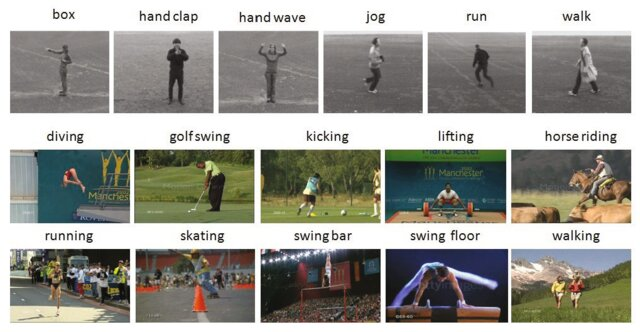
\includegraphics[width=0.8\textwidth]{sample_action_m1}}
	\caption{چندین نمونه از تصاویر فعالیت انسان
		\cite{tasvirAvalChapterYek}
	}
	\label{fig:humanActionM1}
\end{figure}
\subsection{تشخیص فعالیت از نقطه دید انسان}
زمانی که یک اتفاق یا فعالیت که عامل آن انسان است و انسان در به وقوع پیوستن آن عمل نقش دارد را مشاهده می‌کنیم، اولین عاملی که به آن توجه می‌کنیم خود شخص یا موقعیت بدنی شخص است. موقعیت بدنی به عنوان اولین عامل در توجه ما به آن فعالیت یا عمل نقش دارد.

عامل دومی که توجه انسان به آن جلب می‌شود، اشیاء مرتبط با انسان است. برای مثال ممکن است لیوانی که شخص در دست گرفته به ما این مفهوم را القا کند که شخص درحال نوشیدن است. پس اشیاء در فهمیدن یک عمل نقش بسیار مهمی دارند.

عامل بعدی که ناخودآگاه به آن توجه می‌شود، ژست شخص است. برای مثال شخصی درحال دویدن یک ژست و نحوه ایستادن خاصی دارد که انسان با یک نگاه متوجه فعالیتی که شخص درحال انجام آن است می‌شود. این عامل به خصوص در تشخیص فعالیت های ورزشی بسیار مهم است.

شبکه های عصبی عمیق از دل ساختار مغز انسان بیرون آمده و رشد کرده اند. پس طبیعی است که این طرز دید انسان می‌تواند در شبکه های عصبی جای گیرد و باعث شود شبکه درک بهتری از فعالیت داشته باشد. بنابراین از این سه عامل به عنوان عوامل اصلی تشخیص فعالیت انسان در شبکه های عصبی بهره برده می‌شود.

\section{انواع فعالیت های انسان}

فعالیت های انسان به ارتباط بین اشخاص، تعامل با اشیاء و محیطی که درآن زندگی می‌کنیم ربط پیدا می‌کند. این فعالیت ها به اعضای بدن یا حرکات کل بدن اشاره دارد و از چندین عمل ابتدایی که به ترتیب متوالی زمانی انجام می شوند تشکیل شده است. آنها می‌توانند توسط یک فرد یا گروهی از افراد انجام شوند. در این بخش سلسله مراتبی از فعالیت‌های انسانی را بسته به پیچیدگی آنها ارائه می‌شود که از اقدام ساده به رویدادهای پیچیده‌تر مقیاس بندی شده است. شکل
\ref{fig:kinds_human_acions}
این سلسله مراتب را نشان می دهد.

\vspace{8pt}
\begin{figure}[ht]
	\centerline{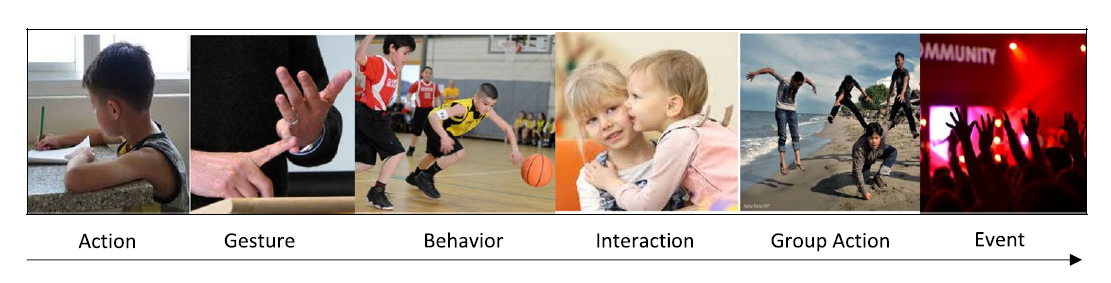
\includegraphics[width=0.8\textwidth]{kinds_human_acions}}
	\caption{انواع فعالیت های انسان از آسان به پیچیده (چپ به راست)
		\cite{HumanActionReviewMogadame}
	}ُ
	\label{fig:kinds_human_acions}
\end{figure}
\begin{itemize}
	\item \textbf{فعالیت اولیه انسان}\\
این شامل فعالیت‌های ساده است که نشان‌دهنده حرکات ارادی و/یا عمدی بدن است که مبنایی برای ایجاد سایر اقدامات پیچیده‌تر مانند «بالا بردن دست چپ» یا «راه رفتن» است. تشخیص این فعالیت ها آسان است و در ابتدا حول این نوع فعالیت ها،‌ تحقیق های زیادی صورت گرفت.
	
	\item \textbf{ژست}\\
 به طور معمول، ژست بخشی از ارتباط غیرکلامی است که می تواند برای بیان ایده ها یا دستورات مهم به کار رود. ژست‌ها نوع دوم فعالیت‌هایی هستند که ممکن است آگاهانه مانند «تشویق کردن» و ناخودآگاه مانند «پنهان کردن صورت با دست هنگام خجالتی شدن» یا «بیرون کشیدن دست هنگام لمس مواد داغ» باشند. برخی از ژست ها جهانی هستند، در حالی که برخی دیگر به زمینه های اجتماعی و فرهنگی کاملاً خاص مربوط می شوند. 
 
 \vspace{10pt}
	\item \textbf{رفتارها}\\
 مجموعه ای از کنش ها و واکنش های فیزیکی افراد در موقعیت های خاص را که از بیرون قابل مشاهده است و با عواطف و حالات روانی آنها مرتبط است، توصیف می کند.

	\item \textbf{فعالیت تعاملی}\\
کنش‌ها یا مبادلات متقابل بین دو نهاد یا بیشتر هستند که رفتار افراد یا اشیاء درگیر در تعامل را تغییر می‌دهند. آنها به طور کلی دو نوع فعالیت پیچیده هستند: انسان به انسان مانند "بوسیدن" یا انسان به شی مانند "آشپزی" که شامل ظروف مختلف در آشپزخانه است.

	\item \textbf{فعالیت گروهی}\\
 فعالیت هایی را تشکیل می دهد که توسط گروهی از افراد انجام می شود مانند "نوازش کردن". این فعالیت ها کم و بیش پیچیده هستند و شناسایی یا تشخیص آنها به دلیل وجود افراز زیاد و شلوغی، دشوار است. 

\end{itemize}

\section{تحلیل موقعیت بدنی در تشخیص فعالیت انسان} 

تحلیل موقعیت بدنی، به عنوان یکی از عوامل اصلی در تشخیص فعالیت انسان در تصاویر، اطلاعات غنی و بی‌نظیری را ارائه می‌دهد. این تحلیل نه تنها موقعیت دقیق دست‌ها و پاها را نشان می‌دهد بلکه به تحلیل زاویه و جهت این اجزاء ارزشمند نیز می‌پردازد. به عبارت دیگر، اطلاعات به دست آمده از تحلیل موقعیت بدنی می‌توانند نقش بسیار موثری در تفسیر رفتار و فعالیت‌های انسانی ایفا کنند.

بررسی مکان قرارگیری پاها و نحوه ایستادن یا حرکت نیز از اهمیت ویژه‌ای برخوردار است. این تحلیل می‌تواند بیشتر اطلاعاتی راجع به نوع فعالیت، مثل ایستادن در یک جا یا حرکت به سمت یک هدف، ارائه دهد. زاویه پاها نیز می‌تواند تصویر کلانی از حرکت انسان در یک لحظه خاص را ارائه کند و به تمیز بین افراد کمک کند.

علاوه بر این، تحلیل موقعیت بدنی به شناخت زاویه و جهت دست‌ها نیز کمک می‌کند. این اطلاعات می‌توانند نشان دهنده اهمیت و چگونگی حرکت دست‌ها باشند، مانند نگه داشتن یک شیء، انجام حرکات آزاد یا انجام حرکات خاص. این اطلاعات ممکن است از انواع فعالیت‌های روزمره مانند نوشیدن یا دست‌کاری با اشیاء گرفته تا فعالیت‌های پیچیده‌تر مثل ورزش‌های ویژه باشد.

نیاز به ترکیب تحلیل موقعیت بدنی با سایر عوامل مانند ژست‌ها و اشیاء از اهمیت خاصی برخوردار است. این ترکیب می‌تواند تفسیرهای دقیق‌تری از رفتار انسانی در تصویر فراهم کند.

در نهایت، تحلیل موقعیت بدنی، با ترکیب اطلاعات مکانی و حرکات اجزاء بدن، به شبکه‌های عصبی عمیق این امکان را می‌دهد تا با دقت بیشتری اقدام به تشخیص فعالیت‌های انسانی در یک تصویر نماید. این تحلیل نه تنها به ارتقاء دقت تشخیص بلکه به بهبود درک از رفتار انسان و نقش آن در تصویر کمک می‌کند.
\section{تحلیل اشیاء مرتبط با انسان در تشخیص فعالیت انسان}
تحلیل اشیاء مرتبط با انسان در تصاویر اطلاعات مهمی را در ارتباط با نوع فعالیت و تعامل انسان با محیط اطراف ارائه می‌دهد. این تحلیل با بررسی نوع و ویژگی‌های اشیاء، امکان تفسیر دقیق‌تر و سودمندتری از فعالیت درحال‌ انجام را فراهم می‌کند. برای مثال، ویژگی‌های یک لیوان در دست انسان می‌تواند نشان‌دهنده فعالیت نوشیدن باشد، در حالی‌که حضور یک دستگاه ورزشی نشان‌دهنده فعالیت ورزشی می‌باشد.
\subsection{تحلیل مکان قرارگیری اشیاء}
ارتباط مکانی اشیاء با انسان نقش اساسی در تعیین تفاوت‌ها و ارتباطات بین انسان و محیط دارد. بررسی مکان وضعیت اشیاء می‌تواند نشان‌دهنده تفصیلاتی از تعاملات و ارتباطات آنها با محیط باشد. به عنوان مثال، حضور یک شال در دست انسان ممکن است نشانگر فعالیتی خاص باشد، مانند خروج در هوای سرد.
\subsection{تمایز بین اشیاء مختلف}
تمایز بین اشیاء مختلف اطلاعات ارزشمندی از نوع و تأثیر اشیاء بر فعالیت انسان ارائه می‌دهد. این تمایز می‌تواند نقش بسزایی در تحلیل تعاملات و تفسیر اثرات مختلف اشیاء داشته باشد. به عنوان مثال، تفاوت میان یک کتاب و یک دستگاه موبایل در دست انسان.
\subsection{ارتباط با اعمال انسان}
بررسی تأثیر اشیاء بر اعمال انسان می‌تواند ما را به سوی درک بهتری از نحوه استفاده و تأثیر اشیاء بر رفتار انسان هدایت کند. این تحلیل می‌تواند نشان‌دهنده نقش یک ابزار ورزشی یا اشیاء کاری باشد که تعامل آن با انسان در تصویر نمایان است.
\subsection{تداخل با اجزاء بدن}
تداخل و تعامل اشیاء با اجزاء بدن اطلاعات اضافی را فراهم می‌کند. این تحلیل می‌تواند ما را به درک بهتری از نحوه استفاده انسان از اشیاء و تأثیر آن بر حرکات بدن هدایت کند. به عنوان مثال، نحوه نگه‌داشتن یک فنجان در دست انسان.
\subsection{ارتباط با دیگر عوامل}
ترکیب تحلیل اشیاء مرتبط با انسان با دیگر عوامل مانند موقعیت بدنی و ژست‌ها امکان تفسیر دقیق‌تر و جامع‌تری از رفتار انسان در تصویر را فراهم می‌کند. این ترکیب می‌تواند به بهبود دقت در تشخیص فعالیت‌های انسانی در تصاویر کمک کند.

تحلیل اشیاء مرتبط با انسان نیز با در نظر گرفتن نقش اشیاء در محیط اطراف انسان، به شبکه‌های عصبی عمیق این امکان را می‌دهد تا با دقت بیشتری نوع فعالیت‌ها و تعاملات انسان با اشیاء را در یک تصویر تشخیص دهد. این تحلیل به گسترش دامنه تفسیر و تشخیص تصاویر کمک کرده و در درک بهتر از فعالیت‌های انسانی در محیط اطراف را نشان می‌دهد. همچنین این تحلیل ما را به سوی یک نگرش جامع تر نسبت به رفتارهای انسانی هدایت می‌کند و اطلاعات ارزشمندی را از جنبه‌های مختلف فیزیکی و روانی ارائه می‌دهد. با پیشرفت تکنولوژی و توسعه الگوریتم‌های هوش مصنوعی، تحلیل ژست‌ها می‌تواند به یک ابزار مؤثر در زمینه‌های مختلف از پزشکی تا رابط‌های کاربری تبدیل شود.
\section{تحلیل ژست در تشخیص فعالیت انسان}
ژست‌ها به عنوان یک جنبه اساسی در تشخیص فعالیت انسان از اهمیت بالایی برخوردارند. تحلیل دقیق این ژست‌ها به ما امکان می‌دهد تا نه تنها نوع فعالیت انسان را شناسایی کنیم بلکه درک عمیق‌تری از رفتارهای جسمی و ذهنی او نیز پیدا کنیم. در ادامه به بررسی اجمالی از تحلیل ژست در تشخیص فعالیت انسان می‌پردازیم و مراحل مختلف این تحلیل را معرفی می‌کنیم.
\subsection{تفکیک ژست‌ها بر اساس نوع فعالیت}
تحلیل ژست‌ها بر اساس نوع فعالیت انسان ابتدا با شناخت پتانسیل پیام‌های مختلف این ژست‌ها شروع می‌شود. به عبارت دیگر، این بخش از تحلیل به درک چگونگی انتقال اطلاعات در جهت تشخیص نوع فعالیت کمک می‌کند. به عنوان مثال، ژستی که به همراه یک وسیله ورزشی صورت گیرد، اطلاعاتی از نوع ورزش درحال انجام را منتقل می‌کند.
\subsection{تحلیل جنبه‌های حرکتی ژست}
در این مرحله، جنبه‌های حرکتی ژست‌ها با دقت بیشتری مورد بررسی قرار می‌گیرند. سرعت، نحوه انجام حرکات، و حتی نقاطی که در طول ژست تاکید شده‌اند، اطلاعات مفیدی در خصوص نحوه اجرای فعالیت انسانی را ارائه می‌دهند. برای مثال، ژست با حرکات متنوع و شتاب‌دار ممکن است به فعالیت ورزشی یا فعالیت‌های پویا اشاره داشته باشد.

\subsection{تحلیل انعکاس ژست در فعالیت}

این مرحله به بررسی انعکاس‌های روحی و فیزیکی ژست‌ها می‌پردازد. انعکاس‌های روحی می‌توانند در بیان حالت هیجانی، شادابی یا حتی استرس شخصیت انسان تاثیرگذار باشند. انعکاس‌های فیزیکی نیز ممکن است جزئیاتی از سلامت و نشاط بدنی را نمایش دهند. این تحلیل به ما کمک می‌کند تا فراتر از سطح ژست، به اطلاعات ضمنی در مورد فعالیت انسانی دست یابیم.

\subsection{تحلیل معناشناسی ژست‌ها}

در این بخش، تحلیل معناشناسی ژست‌ها بیشتر به افق‌های فرهنگی و ارتباطات اجتماعی گسترده می‌شود. هر ژست ممکن است پیام‌های زیادی ارسال کند که باید در سیاق فرهنگ و محیط اجتماعی قرار گیرد. مثلاً، یک ژست معین ممکن است در یک جامعه به معنای احترام و در دیگر جا به معنای خوشحالی باشد. درحالی که درتصویر نمی‌توان تمایزی بین این ها قائل شد لذا این یک عامل انحرافی در شناسایی فعالیت می‌تواند به شمار برود.

\subsection{تفاوت‌ها در ژست‌ها بر اساس فرهنگ}

در این مرحله، تحلیل تفاوت‌های فرهنگی در تشخیص ژست‌ها بررسی می‌شود. هر جامعه و فرهنگ ممکن است ژست‌ها را با تفاوت‌های معنایی خود تفسیر کند. این بررسی به ما کمک می‌کند تا در طراحی سیستم‌های تشخیص ژست، به تفاوت‌های فرهنگی توجه کنیم و جلوی ابهامات در تفسیر ژست‌ها را بگیریم.

\begin{itemize}
	\item
	حال ترکیب سه عامل موقعیت بدنی، اشیاء مرتبط با انسان و ژست به ما این امکان را می‌دهد تا یک تحلیل جامع از فعالیت انسانی داشته باشیم. برای مثال اگر شخصی با یک لیوان در دست، در موقعیت بدنی که نشانگر نشستن است و با ژستی که به حرکات آرامشی اشاره دارد، را مشاهده کنیم، می‌توانیم به احتمال زیاد نتیجه بگیریم که او در حال نشسته و در حال لذت بردن از یک نوشیدنی است. این ترکیب اطلاعات از موقعیت بدنی، اشیاء مرتبط با انسان و ژست به ما اطلاعات دقیق‌تر و گسترده‌تری از فعالیت انسانی ارائه می‌دهد. 
\ref{fig:human_three_amel_mog}
دو نمونه از ارتباط موقعیت بدنی، اشیاء مرتبط و ژست را در فهم فعالیتی که در حال انجام است، نشان می‌دهد. در تصویر سمت  راست"لپ تاپ" و "موس" به عنوان اشیاء، "طرز نشستن افراد" به عنوان ژست و کل ناحیه بدن شخص به عنوان یک موقعیت بدنی نشان می‌دهد که درحال کار با لپ تاپ هستند. در تصویر سمت چپ نیز "لیوان" در تشخیص فعالیت "نوشیدن" و طرز نگه داشتن لیوان در دست نشان می‌دهد که فقط لیوان در دست دارند و درحالی نوشیدن نیستند. پس ژست در اینجا یک عامل کمک کننده است.
\end{itemize}
\vspace{8pt}
\begin{figure}[ht]
	\centerline{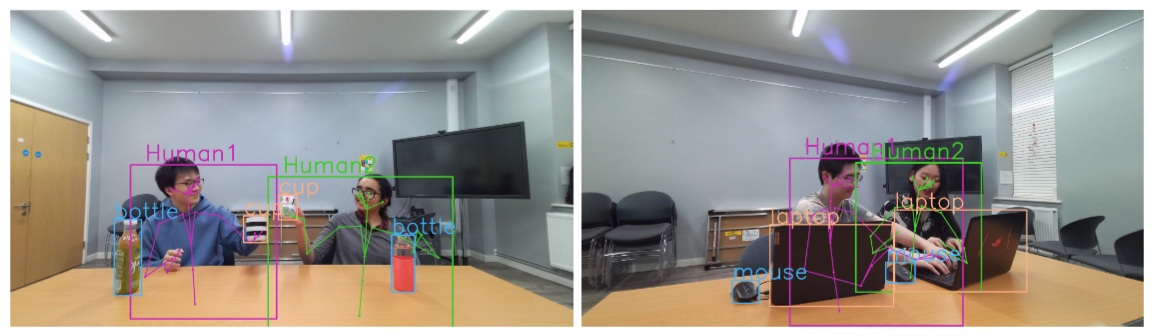
\includegraphics[width=0.8\textwidth]{human_three_amel_mog}}
	\caption{دو نمونه تصویر از تأثیر سه عامل ژست، اشیاء و موقعیت انسان در درک فعالیت
		\cite{tasvirSevomChapterYek}
	}ُ
	\label{fig:human_three_amel_mog}
\end{figure}
\vspace{20pt}

\section{شبکه‌های عصبی عمیق و تشخیص فعالیت انسان در تصویر}

\gls{DeepNeuralNetworks}
 یکی از مفاهیم مهم در زمینه %
\gls{DeepLearning}
  هستند. این ایده از تلاش برای شبیه‌سازی عملکرد مغز انسان و افزایش توانایی یادگیری ماشین در حضور داده‌های بزرگ مشتق شده است.

شبکه‌های عصبی عمیق از ابتدا ایده‌آل محسوب نمی‌شدند ولی با پیشرفت‌های در حوزه پردازش تصویر و صوت، افزایش توانایی محاسباتی، و استفاده از الگوریتم‌های بهبود یافته در آموزش شبکه‌ها، معماری عصبی عمیق به یک ابزار قدرتمند برای حل مسائل یادگیری ماشین تبدیل شده است.

شبکه‌های عصبی عمیق می‌توانند به صورت خودکار و بدون نیاز به تعریف دستی از ویژگی‌ها، اطلاعات مهم را از داده‌ها استخراج کرده و الگوهای مختلف مرتبط با فعالیت‌های انسانی را تشخیص دهند. این مزیت از اهمیت زیادی در حوزه تشخیص و تفسیر تصاویر می‌باشد.

به عنوان مثال، در تشخیص فعالیت انسان در تصاویر، این شبکه‌ها می‌توانند به طور خودکار اجزای مرتبط با افراد، اشیاء، حرکات، و موقعیت‌های مکانی را تشخیص داده و اطلاعات بهتری برای تصمیم‌گیری در مورد نوع فعالیت انسانی فراهم کنند.
استفاده از شبکه‌های عصبی عمیق در این حوزه امکانات جدیدی را برای تحقیقات و کاربردهای عملی فراهم کرده و می‌تواند بهبود قابل توجهی در دقت و کارایی مدل‌ها برای تشخیص فعالیت انسان در تک تصویر داشته باشد. شکل %
\ref{fig:neural_network_action_first}
یک نمونه از چارچوب شبکه عصبی عمیق برای تشخیص فعالیت انسان است. البته دراینجا ورودی چندین سیگنال از فعالیت‌های مختلف است که به شبکه عصبی عمیق داده شده است. درکاربرد مشابه می‌توان ورودی را یک تصویر نیز درنظر گرفت.
\begin{figure}[ht]
	\centerline{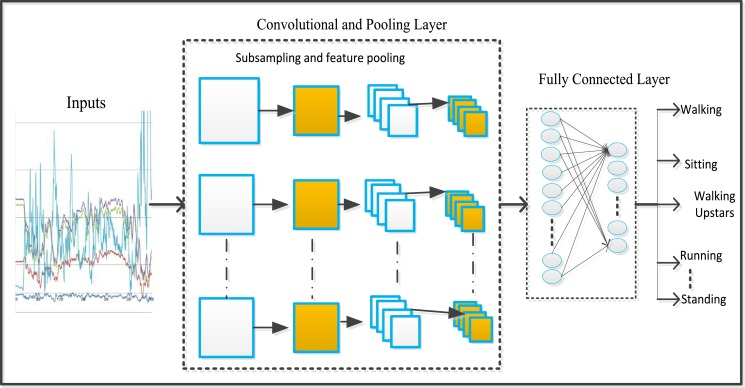
\includegraphics[width=0.7\textwidth]{neural_network_action}}
	\caption{
		مثالی از یک چارچوب شبکه عصبی عمیق برای تشخیص نوع فعالیت
		\cite{WinNT}
	}
	\label{fig:neural_network_action_first}
\end{figure}

در این پایان‌نامه، ما با بهره‌مندی از نقش شبکه‌های عصبی عمیق در فرایند تشخیص فعالیت انسان در تک تصویر به طراحی شبکه و الگوریتم جهت تشخیص فعالیت انسانی، اقدام خواهیم کرد. در زیر به یک سری از مزیت های مهم شبکه‌های عصبی عمیق اشاره شده است:
\begin{itemize}
	\item \textbf{پیچیدگی معماری شبکه‌های عصبی عمیق:}\\
از معماری‌های مختلف شبکه‌های عصبی در این زمینه استفاده می‌شود. معماری مناسب با ویژگی‌های فعالیت‌های انسانی در تصاویر انتخاب و بهینه‌سازی می‌شود. معماری کانوولوشنی%
\LTRfootnote{Convolutional Neural Networks (CNN)}
اغلب در این کاربرد به دلیل استخراج ویژگی‌های متفاوت در سطوح مختلف، مورد استفاده قرار می‌گیرد. 

	\item \textbf{آموزش با %
		\gls{Dataset}
		 متنوع:}\\
آموزش شبکه‌های عصبی عمیق با استفاده از مجموعه داده‌های متنوع و جامع از تصاویر مختلف، از جمله فعالیت‌های انسانی در شرایط مختلف، اطمینان از عملکرد مدل در شرایط واقعی را افزایش می‌دهد.

\item \textbf{قابلیت یادگیری از داده‌های پیچیده:}\\
شبکه‌های عصبی عمیق به عنوان یک الگوریتم یادگیری ماشین با قابلیت یادگیری از داده‌های پیچیده شناخته می‌شوند. این بدان معناست که با تغییرات در شرایط نورپردازی، زاویه دید، وضوح، و تنوع دیگر در تصاویر، این شبکه‌ها قادرند الگوها و ویژگی‌های مفید را به صورت خودکار استخراج کنند.
\end{itemize}

\section{شبکه ترنسفرمر و مکانیزم توجه}

شبکه‌های ترنسفرمر یکی از معماری‌های بسیار قوی در زمینه یادگیری عمیق هستند که ابتدا برای پردازش دنباله‌ها (مثل متون) طراحی شدند.
\cite{AttentionIsAllNeed}
 اما در ادامه، نشان دادند که به عنوان یک راهکار کارآمد می‌توانند در حوزه تشخیص تصاویر و ویدئوها نیز مؤثر باشند. در داخل ترنسفرمر از %
\gls{AttentionMechanism}
استفاده می‌شود.
مکانیزم توجه به شبکه این امکان را می‌دهد تا توجه بیشتری به بخش‌های مهم تصاویر بدهد. این مکانیزم با محاسبه وزن‌های مختلف برای اجزای مختلف تصاویر، اطلاعات مهم را برجسته می‌کند. 

شبکه‌های ترنسفرمر به دلیل قابلیت بررسی دنباله‌های بلند و انتقال اطلاعات بین ورودی‌ها، در تشخیص الگوهای پیچیده مانند فعالیت‌های انسانی در تصاویر مؤثر هستند. این شبکه‌ها با استفاده از لایه‌های توجه، می‌توانند بهترین ویژگی‌ها را از تصاویر استخراج کرده و تمرکز را به بخش‌های مهمتر تصویر معطوف نمایند.

با استفاده از این مکانیزم توجه، حساسیت به جزئیات فعالیت‌های انسانی در تصاویر بهبود یافته و اطلاعات دقیق‌تری در فرآیند تشخیص مورد استفاده قرار می‌گیرد.
شکل%
\ref{fig:transformer_whole_struc}
 ساختار شبکه ترنسفرمر که در کاربرد متن معرفی شده است را نشان می‌دهد. شکل%
\ref{fig:self_attention_struc}
 ساختار
\gls{Self-Attention}
که به عنوان بخش اصلی ترنسفرمر شناخته می‌شود را نشان می‌دهد. هدف از ساختن این نوع معماری مقایسه دوتا بردار باهم است که مشخص شود این دو بردار چقدر با یکدیگر تشابه دارند و به همان میزان باهمدیگر ترکیب شوند تا خروجی معنادار و ارتباط‌دهی شده تولید کند.
\begin{figure}
	\centering
	
	\subfloat[شکل کامل از یک شبکه ترنسفرمر]{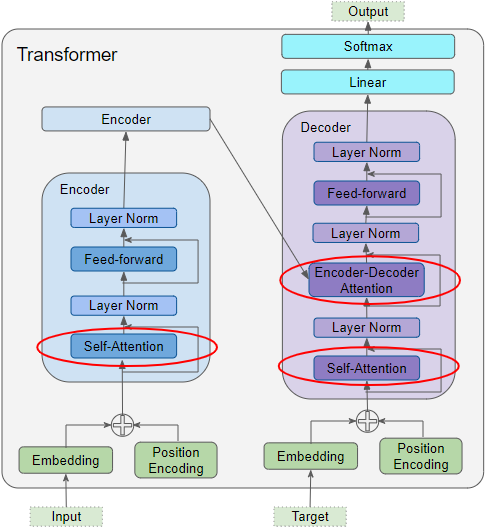
\includegraphics[width=0.5\textwidth]{transformer_whole_struc}\label{fig:transformer_whole_struc}}
	\hfill
	\subfloat[Attention Self داخل ترنسفرمر]{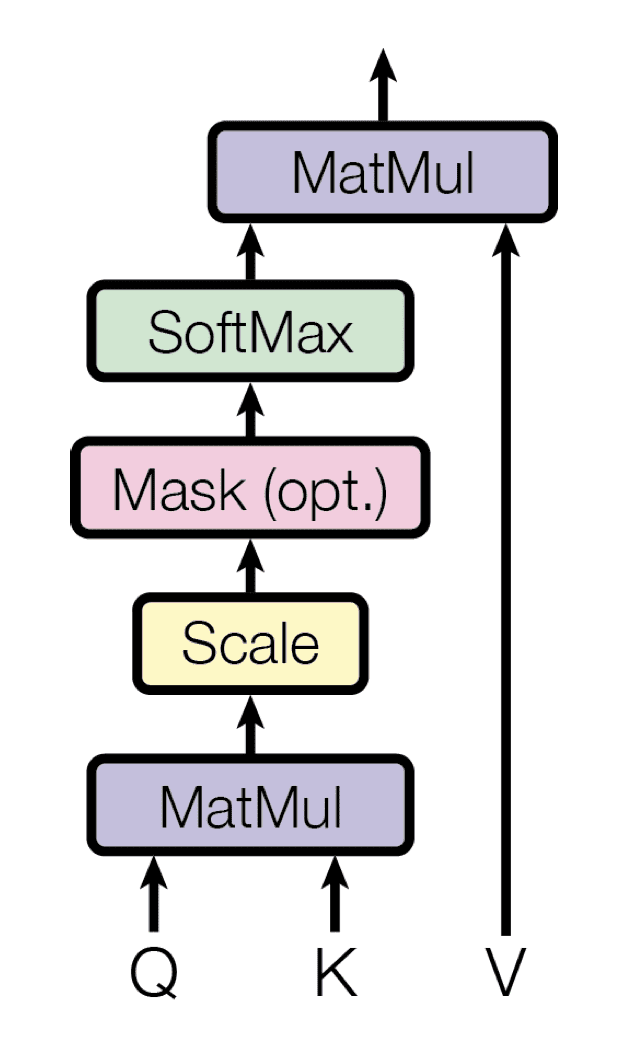
\includegraphics[width=0.3\textwidth]{self_attention_struc}\label{fig:self_attention_struc}}
	
	\caption{ساختار کلی شبکه ترنسفرمر و مکانیزم توجه
		\cite{AttentionIsAllNeed}
	}
	\label{fig:mainfigure}
\end{figure}

\subsection{بهره‌مندی از معماری توجه به خود}

از مکانیزم %
\gls{Self-Attention}
 به عنوان یک ابزار قوی برای تحلیل و استخراج ویژگی‌های تصاویر به منظور شناسایی فعالیت‌های انسانی نیز استفاده می‌شود.
\gls{Self-Attention}
یکی از عناصر اصلی معماری ترنسفرمرها است که توانایی بررسی تمام نقاط ورودی را دارد و در فرایند تصمیم‌گیری بر روی این نقاط تأکید می‌کند.
\gls{Self-Attention}
یک رویکرد در یادگیری عمیق است که به شبکه‌ها این امکان را می‌دهد تا با توجه به اهمیت نقاط مختلف ورودی، وزن‌های مختلفی را به آن‌ها تخصیص دهند.
در مدل %
\gls{Self-Attention}
،هر نقطه ورودی با ویژگی‌های مختلفی از نقاط دیگر ترکیب می‌شود و این امر اطلاعات بسیار غنی‌تری را برای هر نقطه فراهم می‌کند.

\begin{itemize}
	\item \textbf{عملکرد \gls{Self-Attention}در شناسایی فعالیت‌های انسانی}\\
\gls{Self-Attention}
 این امکان را فراهم می‌کند تا شبکه به صورت هوشمندانه بر روی نقاط مهم تصاویر تمرکز کند. این ویژگی می‌تواند در شناسایی افراد، اشیاء، و حرکات مرتبط با فعالیت‌های انسانی بهبود بخشیده و به دقت مدل کمک کند.\\
 همچنین %
\gls{Self-Attention}
  به شبکه این امکان را می‌دهد تا اطلاعات را به صورت همزمان از تمام فضای زمانی تصویر درنظر بگیرد. این ویژگی می‌تواند در تشخیص فعالیت‌های زمانی و توالی‌های مرتبط با انسان کمک کننده باشد. البته چون فعالیت های قابل شناسایی در تک تصویر هستند، به جای توالی‌های زمانی ورودی های دیگری که از تصویر به دست می‌آید را درنظر خواهیم گرفت.
  	\item \textbf{آموزش \gls{Self-Attention}}\\
	\gls{Self-Attention}
  با استفاده از مجموعه داده‌های بزرگ و متنوع، می‌تواند الگوها و اطلاعات مرتبط با فعالیت‌های انسانی را یاد بگیرد. استفاده از یادگیری انتقالی و بهره‌گیری از مدل‌های از پیش‌آموزش دیده شده نیز می‌تواند به بهبود یادگیری در موارد مشابه کمک کند.
    	\item \textbf{ترکیب \gls{Self-Attention} با شبکه های عصبی عمیق}\\
	\gls{Self-Attention}
 به عنوان یک عنصر اصلی در مدل‌های ترنسفرمر، به شبکه‌های عصبی عمیق این امکان را می‌دهد تا در فرایند تصمیم‌گیری و شناسایی فعالیت‌های انسانی از اطلاعات بهتری بهره‌مند شوند.
 ترکیب %
   \gls{Self-Attention}
  با شبکه‌های عصبی عمیق می‌تواند توانایی مدل را در درک و تفسیر تصاویر افزایش دهد و دقت در تشخیص فعالیت‌های انسانی را بهبود بخشد.
\end{itemize}
\section{اهداف پژوهش}
هدف این پایان نامه با درنظر گرفتن موارد گفته شده، تشخیص فعالیت انسان در تصویر می‌باشد که اطلاعات جانبی تصویر در روند تشخیص بکار گرفته می‌شود. این اطلاعات شامل اشیاء مرتبط با فعالیت، ژست انسان و موقعیت بدنی انسان که ناحیه کامل انسان را پوشش است.

در بخش ابتدایی از یک شبکه استفاده می‌شود که ویژگی‌های موجود درتصویر را استخراج کند. این ویژگی‌ها در تعامل با مختصات اشیاء، مختصات ژست و مختصات موقعیت بدنی در یک شبکه ترنسفرمر ترکیب می‌شود که ویژگی‌های مرتبط بهتر مشخص شود. برای توصیف بهتر ژست از مسیر%
\gls{LimbAngleDescriptor}
 استفاده می‌شود که یک بردار توصیف کننده از زاویه اعضای بدن انسان است که یک بردار ویژگی از استخوان بندی%
 \gls{Skeleton}
  بدن را نشان می‌دهد. این مسیر یک مسیر کمک کننده برای شبکه است که از ویژگی‌های نهفته ژست علاوه بر ویژگی‌های ظاهری نیز استفاده شود. هدف نهایی این است که ژست را به نوعی در تشخیص فعالیت دخالت دهیم.

درنهایت مرتبط‌ترین شیء و مرتبط‌ترین ناحیه بدن از ژست انتخاب می‌شود و با خروجی موقعیت بدنی ترکیب می‌شود و یک تشخیص از فعالیت درحال انجام صورت می‌گیرد. پس ورودی شبکه یک تک تصویر و خروجی نهایی یک بردار به طول تعداد دسته‌های موجود در هر مجموعه ‌داده می‌باشد و بسته به تعداد دسته‌بندی‌های مجموعه داده تغییر خواهد کرد. 

ممکن است در برخی از تصاویر کل بدن انسان مشخص نباشد و اصطلاحاً %
\gls{Occlusion}
 رخ دهد که کار تشخیص اعضای بدن انسان را برای تشخیص ژست مشکل می‌کند. برای غلبه براین چالش از ناحیه‌های در دسترس انسان استفاده می‌شود که شبکه ورودی بدون مقدار نداشته نباشد که باعث گمراهی شبکه حین آموزش شود. همچنین شرایط نوری در هرتصویر متفاوت است و ممکن است ناحیه انسان به طور واضح قابل دیدن نباشد، بنابراین یک سری پیش پردازش ها جهت بهبود تصویر انجام می‌شود.

برخی مواقع نیز ممکن است مجموعه داده کافی دردسترس نباشد و شبکه با تکرار آموزش روی این مجموعه داده به سمت %
\gls{Overfitting}
 حرکت کند. درچنین حالتی استفاده از افزایش داده%
 \gls{DataAugmentation}
  مقداری نتیجه را بهبود می‌دهد و همچنین باعث می‌شود شبکه تنوع تصاویر بیشتری به خود ببیند.
\section{سوالات پژوهشی} 
\begin{enumerate}
	\item 
	آیا استفاده از یک شبکه ترنسفرمر در تعامل با مسیر توصیف کننده برای ژست، می‌تواند با استفاده از مختصات ژست مدل مناسبی برای تشخیص فعالیت انسان باشد؟
	\item
	با توجه به چالش‌های شناسایی نقاط کلیدی بدن در تک تصاویر، کدام یک از نقاط کلیدی انسان در شناسایی ژست تاثیر کمتری داشته و می‌‌تواند نادیده گرفته شود؟
	\item
	آیا استفاده از ژست انسان و ترکیب آن با ویژگی ظاهری انسان می‌تواند منجربه افزایش دقت در شناسایی نوع فعالیت انسان گردد؟
	\item
	آیا استفاده از اطلاعات مکانی اشیاء و موقعیت و نوع آنها نسبت به مکان انسان در تصویر می‌تواند منجر به افزایش دقت در شناسایی نوع فعالیت انسان گردد؟
\end{enumerate}
\section{جمع بندی و ارائه راهکار پیشنهادی} 

طبق مواردی که گفته شد هدف این پایان نامه، تشخیص نوع فعالیت انسان در تصویر است. در تصویر به دلیل نبودن اطلاعات زمانی شناسایی عمل چالش هایی دارد. گفتیم که انسان به صورت ذاتی می‌تواند بسیاری از فعالیت‌های درحال انجام را حتی از روی تصویر تشخیص دهد.

سپس به انواع فعالیت‌های انسانی پرداختیم که سطح بندی های متفاوتی دارد. از فعالیت های اولیه که شامل حرکات ابتدایی انسان مانند راه رفتن،‌ دویدن و... است، تا در آخر که فعالیت های پیچیده مانند یک مهمانی که درافراد زیادی در به وقوع پیوستن این فعالیت مشارکت دارند، اشاره شد.

درادامه به نحوه تشخیص فعالیت های انسانی از روی موقعیت بدنی شخص، اشیاء مرتبط با انسان و ژست شخص قابل شناسایی است،‌ پرداخته شد و انواع آنها نام برده شد و ترکیب اشیاء، ژست و موقعیت بدنی انسان برای تشخیص فعالیت درنظرگرفته شد. شبکه های عصبی و مکانیزم توجه به صورت مختصر توضیح داده شد که به چه صورت در کاربرد شناسایی فعالیت می‌توان بهره‌مند شد.

تشخیص فعالیت انسان از روی تک تصویر،‌ یک مسئله %
\gls{Classification}
 محسوب می‌شود بنابراین از بیشتر الگوریتم ها و ارزیابی‌های مرتبط با طبقه‌بندی دراین کار استفاده می‌شود. معماری پیشنهادی در این پایان استفاده از یک شاخه‌ی دیگر از %
 \gls{Self-Attention}
  به منظور ترکیب ویژگی‌های موقعیت بدنی با ژست انسان است. در این حالت اجزای بدن به صورت جداگانه با کل تصویر فرد ترکیب می‌شود و شبکه به یک درکی از ژست می‌رسد که در شناسایی فعالیت تاثیرگذار است.
  
 به دلیل محدود بودن سیستم محاسباتی و طولانی بودن زمان آموزش و همچنین پیچیدگی محاسباتی زیاد تشخیص فعالیت در ویدیو،‌ ما سراغ تشخیص فعالیت در تک تصویر رفتیم. هدفمان این است که از داده‌ها و اطلاعات موجود استفاده کنیم تا نشان دهیم ترکیب ژست با عواملی مانند موقعیت بدنی چه نتایجی می‌تواند داشته باشد و آیا درنظر گرفتن این فاکتور موجب افزایش دقت می‌شود یا نه.

\section{ساختار پایان نامه} 

فصل دوم مروری از کارهایی که در این زمینه انجام شده، بررسی می‌شود و به بررسی چهار زیرشاخه اساسی از تشخیص تصویر محور پرداخته شده است.

پس از بررسی کارهای گذشته، در فصل سوم روش پیشنهادی بررسی می‌شود. دراین مرحله از پیش پردازش‌ها شروع شده و پس از بررسی آنها به دو روش اصلی استفاده از ژست پرداخته می‌شود و هرکدام از آنها را در قالب یک بخش جداگانه بررسی می‌کنیم.

در فصل چهارم نتایجی که از ارزیابی روش پیشنهادی درمقایسه با یک سری کارهای اصلی گزارش می‌شود. روی دو نمونه از مجموعه ‌داده‌هایی که اغلب در این خوزه کاربرد دارند تست و اجزا می‌شود و نتایج هرکدام در بخش جداگانه گزارش می‌شود.

در فصل آخر نیز به نتیجه‌گیری نهایی و پیشنهادات برای کارهای آتی پرداخته می‌شود.

